\documentclass[default]{beamer}
\setbeamertemplate{navigation symbols}{}

\usetheme{Boadilla}
%\usecolortheme{beaver}
%\usetheme{default}
%\useoutertheme{infolines}


\usepackage[utf8]{inputenc}					% Выбор языка и кодировки
\usepackage[english,russian]{babel}	% Языки: русский, английский
\usepackage{csquotes}

\usepackage{tikz}
\usetikzlibrary{arrows,shapes,calc}
\everymath{\displaystyle}
\tikzstyle{every picture}+=[remember picture]

\usepackage{animate}
\usepackage{fp}
\usepackage{textpos}

\usepackage[
	language=auto,
	autolang=other,
	backend=biber,
	style=authortitle,
	sorting=ydnt,
	maxbibnames=5
]{biblatex}
\addbibresource{panov_rcai2018.bib}
				
\DeclareSourcemap{
	\maps[datatype=bibtex, overwrite]{
		\map{
			\step[fieldset=langid, fieldvalue=english]
			\step[fieldset=doi, null]
			\step[fieldset=issn, null]
			\step[fieldset=isbn, null]
			\step[fieldset=url, null]
			\step[fieldsource=language, fieldset=langid, origfieldval]
		}
	}
}
\DeclareBibliographyDriver{std}{%
	\usebibmacro{bibindex}%
	\usebibmacro{begentry}%
	\usebibmacro{author/editor+others/translator+others}%
	\setunit{\labelnamepunct}\newblock
	\usebibmacro{title}%
	\newunit\newblock
	\usebibmacro{maintitle+booktitle}
	\newunit\newblock
	\usebibmacro{journal}%
	\newunit\newblock
	\usebibmacro{date}%
	\newunit\newblock
	\usebibmacro{finentry}
}
\DeclareBibliographyAlias{article}{std}
\DeclareBibliographyAlias{book}{std}
\DeclareBibliographyAlias{inproceedings}{std}
\DeclareBibliographyAlias{incollection}{std}

\graphicspath{{../../images/}} 			% Пути к изображениям

\makeatletter
\setbeamertemplate{footline}
{
	\leavevmode%
	\hbox{%
		\begin{beamercolorbox}[wd=.333333\paperwidth,ht=2.25ex,dp=1ex,center]{author
				in head/foot}%
			\usebeamerfont{author in
				head/foot}\insertshortauthor~~\beamer@ifempty{\insertshortinstitute}{}{(\insertshortinstitute)}
		\end{beamercolorbox}%
		\begin{beamercolorbox}[wd=.333333\paperwidth,ht=2.25ex,dp=1ex,center]{title in
				head/foot}%
			\usebeamerfont{title in head/foot}\insertshorttitle
		\end{beamercolorbox}%
		\begin{beamercolorbox}[wd=.333333\paperwidth,ht=2.25ex,dp=1ex,right]{date in
				head/foot}%
			\usebeamerfont{date in head/foot}\insertshortdate{}\hspace*{1em}
			\insertframenumber{}\hspace*{2ex} 
		\end{beamercolorbox}
	}%
	\vskip0pt%
}

\addtobeamertemplate{frametitle}{}{
	\begin{textblock*}{100mm}(\textwidth-35pt,-15pt)
		\includegraphics[height=5mm]{misc/logos/frccsc140.png}
		\includegraphics[height=5mm]{misc/logos/mipt_en.jpg}
	\end{textblock*}
}

\renewcommand*{\bibfont}{\tiny}
\setlength\bibitemsep{-5pt}
\newcommand{\predmatr}[3]{
	\node[ell, rectangle, minimum height = 15, minimum width = 7.5]  at (#1 pt,#2 pt) {}; 
	\node[ellf, rectangle, minimum height = 15, minimum width = 7.5] at (#1+7.5 pt,#2 pt) {};
	\node[minimum height = 15, minimum width = 15] (#3) at (#1+3.3pt,#2 pt) {};
	\draw[ell] (#1+7.5 pt,#2+7.5 pt) -- (#1 +7.5 pt,#2-7.5 pt);
}
\begin{document}
	
	\title[Cognitive dynamic systems]{Cognitive dynamic systems}
	\author[Aleksandr I. Panov]{Aleksandr I. Panov}
	\institute[RAS]{Federal Research Center ``Computer Science and Control''\\Russian Academy of Sciences (RAS)\\Moscow Institute of Physics and Technology\\\textbf{Moscow}}
	\date[September 25 -- RCAI 2018]{September 25 -- RCAI 2018} 
		
	\begin{frame}
		\titlepage
		\centering
		
\includegraphics[height=20pt]{misc/logos/ras_en.png} \hspace{10pt}
		
\includegraphics[height=20pt]{misc/logos/frccsc.png} \hspace{10pt}
		\includegraphics[height=20pt]{misc/logos/mipt_en.jpg}
	\end{frame}

	\begin{frame}
		\frametitle{Outline}
		\tiny
		\tableofcontents
	\end{frame}

	\section{Cognitive dynamic systems (CDS): Background}
	\subsection{Intelligent dynamic systems}
	\begin{frame}{Rule-based DIS}
		\begin{itemize}
			\item Rule is the triple $r=\left\langle C,A,D \right\rangle$.
			\item The set of rules $\Pi $ is divided into two subsets ${{\Pi }_{CL}}$  and ${{\Pi }_{TR}}$:
			\begin{align*}
			& {{\Pi }_{CL}}=\left\langle C\left( t \right),A\left( t \right),D\left( t \right) \right\rangle , \\ 
			& {{\Pi }_{TR}}=\left\langle C\left( t \right),A\left( t+1 \right),D\left( t+1 \right) \right\rangle .
			\end{align*}
			\item Closure and transition functions:
			\begin{align*}
			& \Phi \left( \chi \left( t \right) \right)=\left( CL,\chi \left( t \right) \right):{{2}^{X}}\to {{2}^{X}},\\
			& \Psi \left( \chi \left( t \right),t \right)=\left( TR,\chi \left( t \right),t \right):{{2}^{X}}\times T\to {{2}^{X}}.
			\end{align*}
			\item A quadruple $D=\left\langle X,T,\Phi ,\Psi  \right\rangle $ is called an intelligent rules-based dynamic system.
		\end{itemize}
		
		\vspace{-5pt}
		\nocite{*}
		\printbibliography[keyword={dis}, resetnumbers=true]
	\end{frame}
	\begin{frame}{DIS tasks}
		\begin{itemize}
			\item Generation of the goal-driven behavior.
			\item Trajectory stability issues.
			\item Synthesis of control to compensate for disturbances.
			\item Synthesis of feedback.
			\item General issues of dynamic systems controllability.
		\end{itemize}
		
		\par\bigskip
		\nocite{*}
		\printbibliography[keyword={dis}, resetnumbers=true]
	\end{frame}

	\subsection{Unresolved issues}
	\begin{frame}{Goal-setting problem}
		\begin{center}
			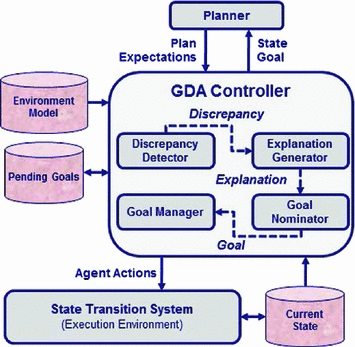
\includegraphics[width=0.4\textwidth]{misc/control/gda.jpg}
		\end{center}
		\scriptsize
		For example GDA performs goal reasoning in four tasks: 
		\begin{itemize}
			\item discrepancy detection,
			\item explanation, 
			\item goal formulation, 
			\item goal management.
		\end{itemize}
		
		\par\bigskip
		\nocite{*}
		\printbibliography[keyword={gda}, resetnumbers=true]
	\end{frame}
	\begin{frame}{Role distribution problem}
		\begin{itemize}
			\item Agents solve a common problem (have a common top-level goal).
			\item Agents act independently (decentralized control), including the ability to set individual sub-goals and achieve them.
			\item Agents have different characteristics, both technical and cognitive, i.e. different strategies of behavior.
			\item Agents possess different knowledge bases.
			\item Agents operate in a dynamic environment.
		\end{itemize}
		
		\par\bigskip
		\nocite{*}
		\printbibliography[keyword={roles}, resetnumbers=true]
	\end{frame}
	\begin{frame}{Symbol grounding problem}
		\begin{center}
			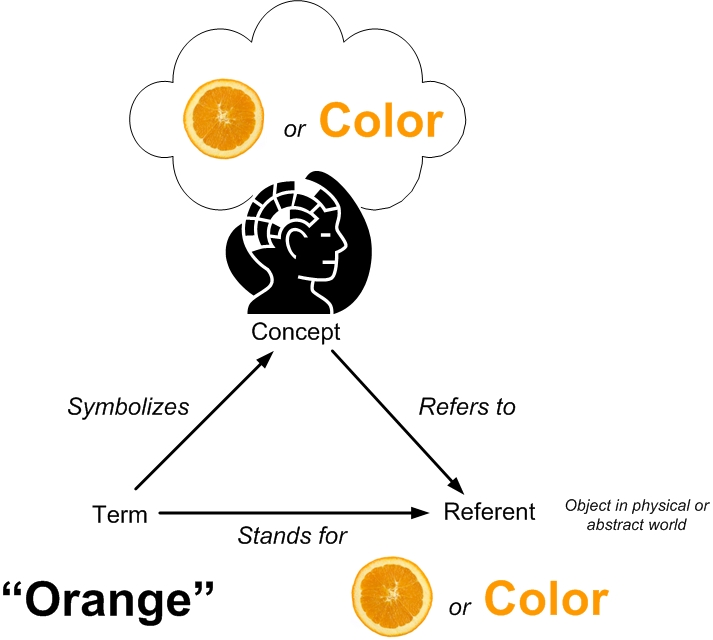
\includegraphics[width=0.4\textwidth]{signs/symb_ground.jpg}
		\end{center}
		\small
		Classical methods of artificial intelligence are symbolic (logic, set of rules, planning, learning). However, thinking --- is more than symbol manipulation.
		\par\medskip
		This problem is especially relevant in robotics (\textbf{symbol anchoring}) --- the system should learn symbols based on its own experience.
				
		\par\bigskip
		\nocite{*}
		\printbibliography[keyword={sgp}, resetnumbers=true]
	\end{frame}
	
	\subsection{Integration of ideas from psychology and neurophysiology}
	\begin{frame}{Psychology and Neurophysiology}
		\begin{itemize}
			\item Various applications that require or prefer human-like behaviour and performance.
			\item Cognitive architectures may serve as a good basis for building mind/brain-inspired, psychologically realistic cognitive agents.
			\item ``Cognitive synergy'', wherein different components are specifically integrated in such a way as to compensate for each others scalability weaknesses.
			\item Bridging the gap between neurophysiological realities and mathematical and computer science concepts.
		\end{itemize}
		
		\par\bigskip
		\nocite{*}
		\printbibliography[keyword={agi}, resetnumbers=true]
	\end{frame}
	
	\subsection{Applied semiotics: knowledge representation}
	\begin{frame}{Knowledge representation as a main issue of AI}
		\begin{itemize}
			\item Knowledge representation approaches vs machine learning approaches.
			\item Representing knowledge in order to design formalisms that will make complex systems easier to design and build. 
			\item Knowledge representation and reasoning also incorporate findings from logic to automate various kinds of reasoning.
		\end{itemize}
		
		\par\bigskip
		\nocite{*}
		\printbibliography[keyword={finn}, resetnumbers=true]
	\end{frame}
	\begin{frame}{Applied semiotics by Pospelov}
		\small
		Semiotic knowledge bases:
		\begin{itemize}
			\item \textbf{Naming}: information unit, which purports to be knowledge, needs to have some tag - name.
			\item \textbf{Structuring}: an information unit must have its own internal structure.
			\item \textbf{Principle of ``matryoshka''}: signs are embedded into each other through inheritance relationships, providing a description of entities at different levels.
			\item \textbf{Connectivity}: the signs due to the different relations are combined in the network.
			\item \textbf{Activity}: in sign networks it becomes possible to implement the principle of ``knowledge activation is source of procedures activation''.
			\item \textbf{Reflexivity}: the appearance of the meta-level allows the system to talk about itself, about the nature of its information about the world.
		\end{itemize}

		\nocite{*}
		\printbibliography[keyword={semiotics}, resetnumbers=true]
	\end{frame}

	\section{Psychological evidences}
	\subsection{Theory of activity $\rightarrow$ actions}
	\begin{frame}{Theory of activity by Leontyev}
		\begin{columns}
			\begin{column}{0.4\textwidth}
				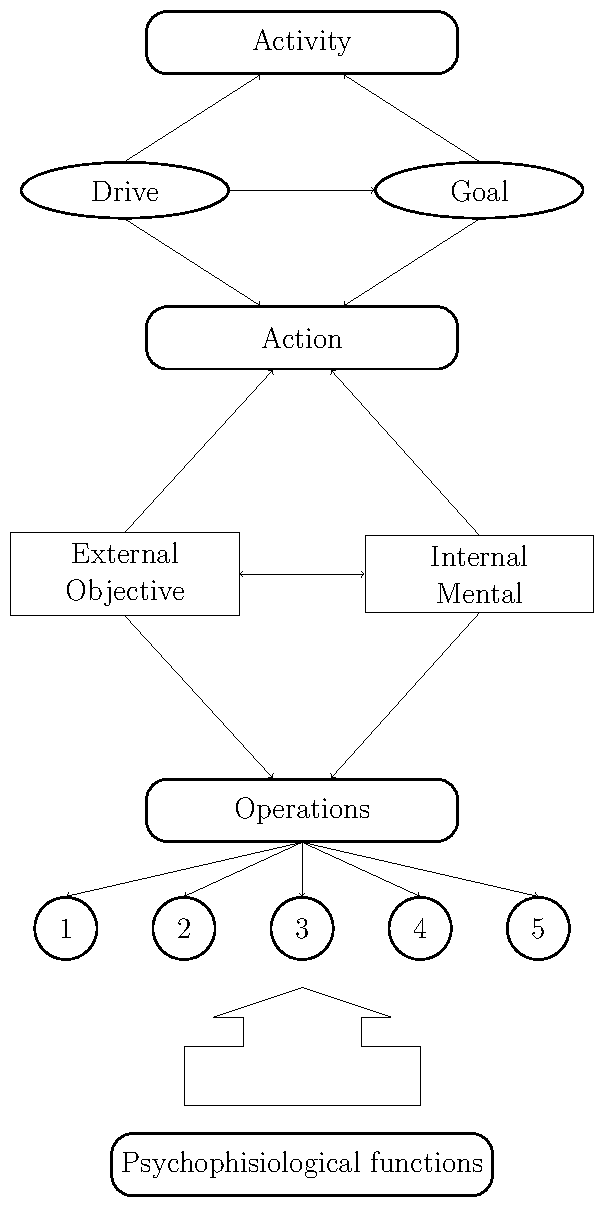
\includegraphics[width=0.7\textwidth]{misc/psycho/activity_en.pdf}			
			\end{column}
			\begin{column}{0.6\textwidth}
				\begin{center}
					\includegraphics[width=0.17\textwidth]{misc/photos/leontyev.jpg}
				\end{center}
				Base concepts:
				\begin{itemize}
					\item Human behavior is a dual hierarchical structure of motives-goals and actions-operations.
					\item Activity is an active, purposeful process.
					\item Human actions are subject; their goals are social in nature.
					\item Consciousness and activity are inextricably linked.
				\end{itemize}
			\end{column}
		\end{columns}
		\par\bigskip
		\nocite{*}
		\printbibliography[keyword={activity}, resetnumbers=true]
	\end{frame}

	\subsection{Cultural-historical approach $\rightarrow$ communication}
	\begin{frame}{Cultural and historical approach by Vygotsky}
		\begin{center}
			\includegraphics[width=0.15\textwidth]{misc/photos/vygotsky.jpg}
		\end{center}
		\scriptsize
		Theory of origin and development of higher mental functions:
		\begin{itemize}
			\item \textbf{Social environment} --- the main source of personality development.
			\item Mastery of culture, ways of behavior and thinking.
			\item The development of cognitive functions occurs primarily through the child's using of \textbf {``psychological tools''}, by mastering the system of character signs, such as language, writing, counting.
			\item External activity, when cultural tools are subject, as mining collapses (\textbf{interiorized}) in the internal plan.
			\item In the first stage of external activity the child does everything in \textbf{cooperation} with adults - ``zone of proximal development''.
			\item The development is not exactly gradual, and \textbf{multi-stage} process.
			\item Consciousness develops through the \textbf{dialogue}: a child's dialogue with an adult or an adult's dialogue with an adult.
		\end{itemize}
	\end{frame}

	\begin{frame}{Sign as a tool of mental activity}
		\begin{center}
			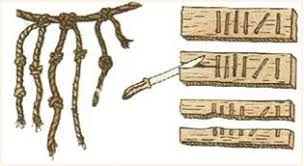
\includegraphics[width=0.4\textwidth]{misc/psycho/link.jpg}
		\end{center}
		
		\begin{itemize}
			\item Sign is a hand-made stimulus, a means to control one's behavior and the behavior of others.
			\item The history of human development is the history of the sign: the more developed the system of signs in the generation, the more developed the higher mental functions.
			\item Signs: rock art, signs, gestures, speech, notes, etc.
		\end{itemize}
		\par\bigskip
		\nocite{*}
		\printbibliography[keyword={vygotsky}, resetnumbers=true]
	\end{frame}

	\subsection{Structure of the sign}
	\begin{frame}{Three elements of the sign-based world model}
		\footnotesize
		\begin{figure}
			\includegraphics[width=0.3\textwidth]{signs/en/sign_colored_rita}
		\end{figure}
		
		We present an entity as three cause-effect (causal) structures:
		\begin{itemize}
			\item {\color{red}image structure} - representation of the relationship of external signals and internal characteristics of the subject (agent) - sensorimotor representation,
			\item {\color{blue}value structure} - generalized knowledge of relations in the outside world, agreed in some group of subjects (agents),
			\item {\color{green!60!black}the structure of the personal meaning} - situational requirement of motivational interpretation of knowledge about the relationships in the external environment (``the value for me'').
		\end{itemize}
	
		\nocite{*}
		\printbibliography[keyword={qualia}, resetnumbers=true]
	\end{frame}
	
	\subsection{Related works: cognitive architectures}
	\begin{frame}{Cognitive architectures}
		\begin{center}
			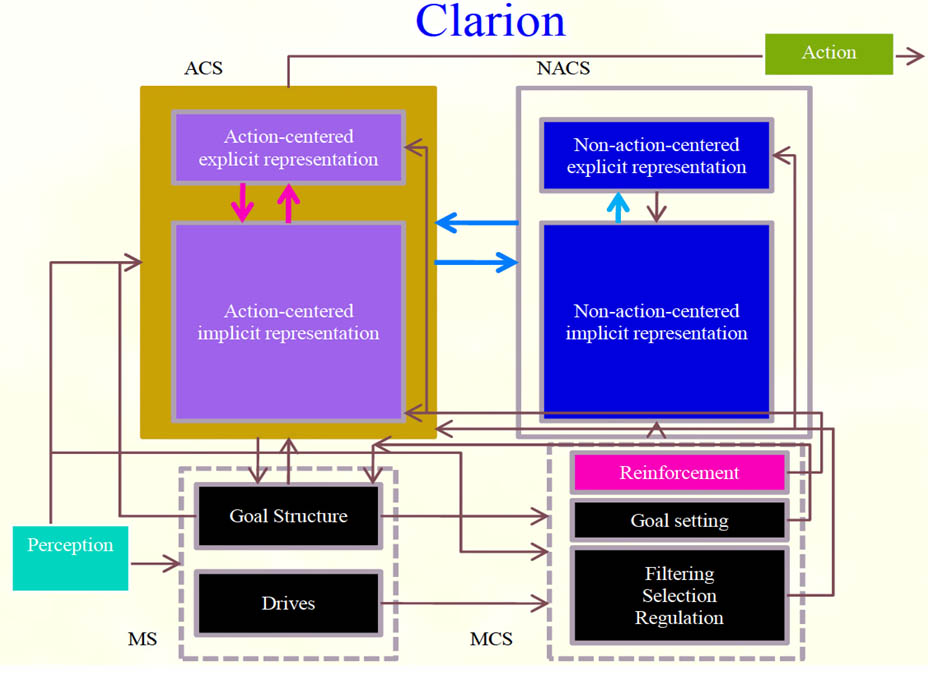
\includegraphics[width=0.3\textwidth]{agent-schemas/en/clarion.jpg}
			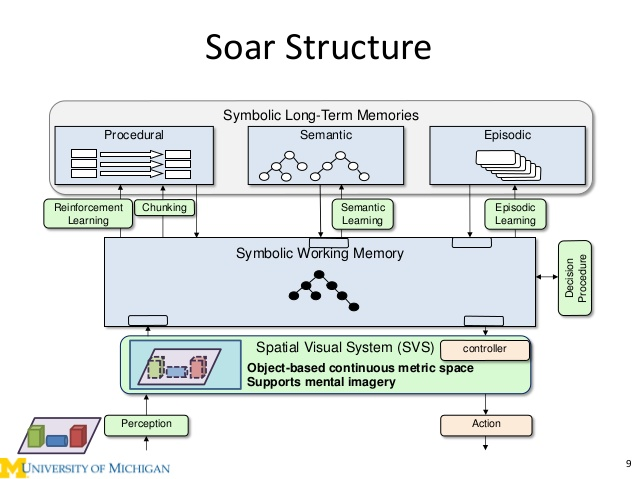
\includegraphics[width=0.3\textwidth]{agent-schemas/en/soar.jpg}
		\end{center}
		\scriptsize
		Disadvantages of modern cognitive architectures:
		\begin{itemize}
			\item The conceptually unresolved problems of binding symbols (symbol grounding problem) - CLARION.
			\item The lack of the activity model of the system behavior, there is implementation of only some cognitive aspects
			\item Hierarchy of knowledge representations (4D/RCS).
			\item The possibility of implementing a hierarchical planning.
			\item Implementation of conceptual knowledge learning - Cognitive Mario.
			\item Modeling of the reflexive behavior.
		\end{itemize}
		\vspace{-5pt}
		\nocite{*}
		\printbibliography[keyword={symbgrnd}, resetnumbers=true]
	\end{frame}
	
	\section{Neurophysiological evidences}
	\subsection{Perception cycle: Ivanitsky and Edelman}
	\begin{frame}{Three elements of the sign-based world model}
		\begin{figure}
			\includegraphics[width=0.45\textwidth]{misc/phisio/ivan_cyrc_en}
			\quad
			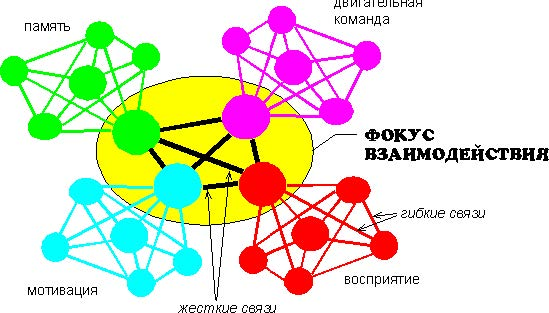
\includegraphics[width=0.45\textwidth]{misc/phisio/focus_inter.jpg}
		\end{figure}
		\small
		A.Ivanitsky (\textit{information synthesis}), G.Edelman (\textit{theory of re-entry}):  the emergence of sensations, i.e. activation of some element of the personal knowledge, occurs with the closure of contour of the nervous excitement distribution from the sensory input. The value of the signal (the hippocampus) and emotional relations (hypothalamus) impose on the received sensory information.
		
		\nocite{*}
		\printbibliography[keyword={ivan}, resetnumbers=true]
	\end{frame}

	\subsection{Global workspace theory}
	\begin{frame}{Three elements of the sign-based world model}
		\begin{figure}
			\includegraphics[width=0.35\textwidth]{misc/phisio/workspace}
		\end{figure}
		
		\scriptsize
		\begin{itemize}
			\item Conscious cognitive content is globally available for diverse cognitive processes including attention, evaluation, memory, and verbal report.
			\item Global availability is necessarily limited to a single stream of content.
			\item Sensory stimuli mobilize excitatory neurons with long-range cortico-cortical axons, leading to the genesis of a global activity pattern among workspace neurons.
			\item Any such global pattern can inhibit alternative activity patterns among workspace neurons.
		\end{itemize}
		\vspace{-5pt}
		\nocite{*}
		\printbibliography[keyword={baars}, resetnumbers=true]
	\end{frame}
	\subsection{Mountcastle and Hawkins}
	\begin{frame}{Structural homogeneity}
		
		\begin{columns}
			\begin{column}{0.35\textwidth}
				\includegraphics[width=0.8\textwidth]{misc/phisio/mozg_2}
				\par\bigskip
				\hspace{-7mm}\includegraphics[width=\textwidth]{misc/phisio/mozg}
			\end{column}
			\begin{column}{0.65\textwidth}
				\includegraphics[width=\textwidth]{misc/phisio/cortex_layers}
			\end{column}
		\end{columns}
		\nocite{*}
		\printbibliography[keyword={column}, resetnumbers=true]
	\end{frame}
	\begin{frame}
		\frametitle{An elementary unit}
		\scriptsize
		
		\begin{center}
			\includegraphics[width=0.35\textwidth]{misc/mpf/hawkins_htm}
			\includegraphics[width=0.3\textwidth]{misc/mpf/hawkins_htm_ex_a}
			\includegraphics[width=0.3\textwidth]{misc/mpf/hawkins_htm_ex_b}
		\end{center}
		The main principles of the learning mechanism are: 
		
		\begin{itemize}
			\item using a hierarchy of computing nodes with bottom-up and top-down streams, 
			\item using Hebbian rules for learning, 
			\item separation of spatial and temporal poolers, 
			\item suppression of secondary activation for the formation of sparse representations.
		\end{itemize}
		\vspace{-5pt}
		\nocite{*}
		\printbibliography[keyword={htm}, resetnumbers=true]
	\end{frame}
	\subsection{Related works: NeSy}
	\begin{frame}
		\frametitle{Neural symbolic computation}
		
		\begin{center}
			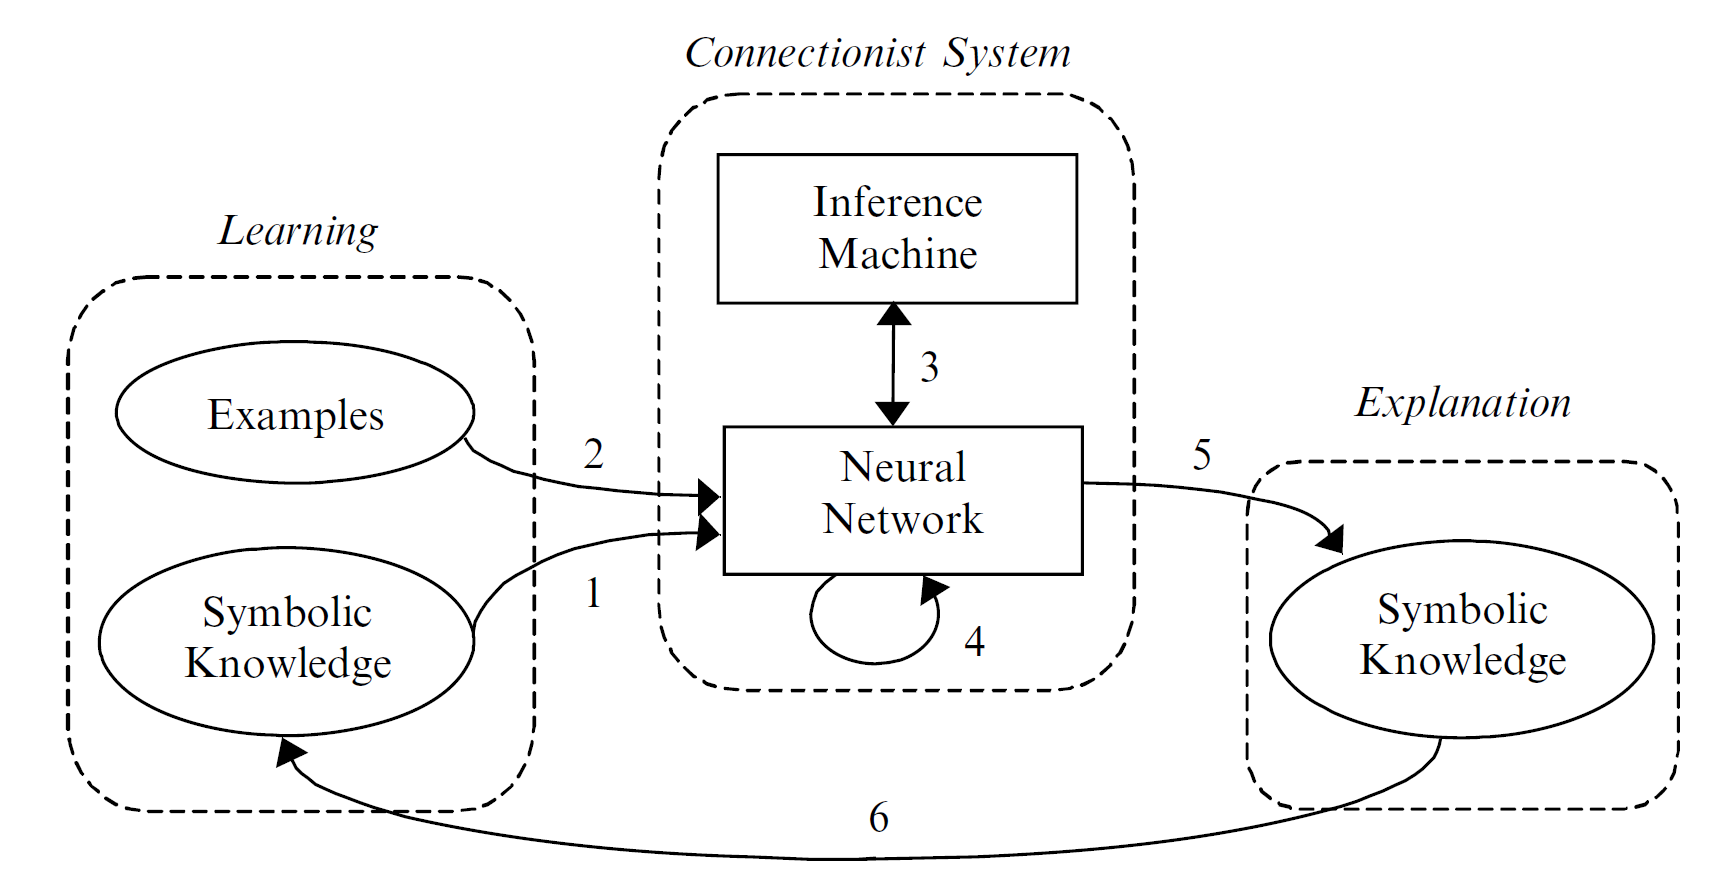
\includegraphics[width=0.45\textwidth]{misc/signs/neuro_symb.png}
		\end{center}
		\textbf{Basic idea}: encoding a symbol by a vector of numbers and then representing that vector by links in an ensemble of artificial neurons (embedding).
		\par\medskip
		\textbf{The main result}: by introducing special rules on the distribution of activity in neural networks some simple logic circuits are implemented.
		\par\medskip
		\textbf{Main drawback}: limited integration of learning.
		
		\nocite{*}
		\printbibliography[keyword={neuro_symb}, resetnumbers=true]
	\end{frame}


	\section{Synthesis}
	\subsection{Base definitions: sign, semiotic network, cognitive function}
	\begin{frame}{Causal matrix}                             
		\begin{center}
			\includegraphics[width=0.6\textwidth]{causnet/caus_matr}
		\end{center}
		
		\vspace{-5pt}
		\nocite{*}
		\printbibliography[keyword={matrix}, resetnumbers=true]
	\end{frame}
	\begin{frame}{Causal tensor}                             
		\begin{center}
			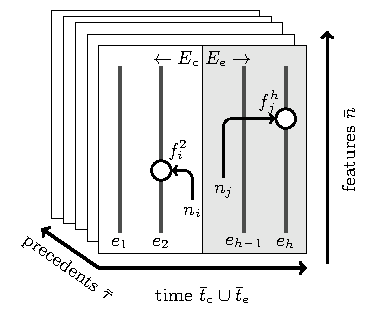
\includegraphics[width=0.4\textwidth]{causnet/caus_tensor_en}
		\end{center}
		
		A causal tensor $T (n)=T[n,\bar{n}, {{\bar{t}}_{c}},\bar{\tau }]$ is a three-dimensional array of real numbers of dimension $r\times q\times h$, which is provided with an identifier $n$ and three reference vectors: 
		\begin{itemize}
			\item an indicative vector $\bar{n}=({{n}_{1}},{{n}_{2}},..., {{n}_{q}})$; 
			\item a temporary vector ${{\bar{t}}_{c}}=({{t}_{1}},{{t}_{2}},...,{{t}_{{{h}_{c}}}})$; 
			\item a case vector $\bar{\tau } =({{\tau }_{1}},{{\tau }_{2}},..., {{\tau }_{r}})$.
		\end{itemize}

	\end{frame}
	
	\begin{frame}{Causal network}    
		\small                         
		Causal network $W=(\mathbf{T},\mathbf{L})$ is a directed labeled multigraph where the set of vertices $\mathbf{T}$ with the tags $\{{{n}_{1}},{{n}_{2}},...\}$ corresponds to the set of causal tensors $\{T({{n}_{1}}),T ({{n}_{2}}),\dots\}$ and set of arcs $\mathbf{L}$ consists of arcs ${{l}_{i}}=T({{n}_{i}})\to T({{n}_{j}})=(T[{{n}_{i}},{{\bar{n}}_{i}},{{\bar{t}}_{ci}},{{\bar{\tau }}_{i}}],T[{{n}_{j}},{{\bar{n}}_{j}},{{\bar{t}}_{cj}},{{\bar{\tau }}_{j}}])$ such that ${{n}_{i}}\in {{\bar{n}}_{j}}$, and marked by triplet $\{{{\varepsilon }_{1}},{{\varepsilon }_{2}},{{\varepsilon }_{3}}\}$ where
		\begin{itemize}
			\item ${{\varepsilon }_{1}}={{\tau }_{k}}$ such that ${\tau}_{k}\in {\bar{\tau }}_{j}$ and $\exists {{e}_{u}}=(f_{1}^{u},f_{2}^{u},\dots,f_{q}^{u})\in {{E}_{c}} ({n}_{j})\cup {{E}_{e}} ({n}_{j})$, in which $\exists f_{v}^{u}>{{\theta}^{f}}$, that is, this label corresponds to such a precedent in the tensor $T({{n}_{j}})$ for which an event exists in the causal matrix in which the tensor-trait $T({{n}_{i}})$ manifests itself with a value above the threshold ${{\theta }^{f}}$;
			\item ${{\varepsilon}_{2}}={{t}_{k}}$ so ${{t}_{k}}>0$ then ${{t}_{k}}\in {{\bar{t}}_{cj}}$ and  ${{e}_{{{t}_{k}}}}=(f_{1}^{{{t}_{k}}},f_{2}^{{{t}_{k}}},\dots,f_{q}^{{{t}_{k}}})\in {{E}_{c}} ({{n}_{j}})\cup {{E}_{e}}({{n}_{j}})$ exists $f_{v}^{{{t}_{k}}}>{{\theta }^{f}}$ and if ${{t}_{k}}<0$, then ${{t}_{k}}\in {\bar{t}_{ej}}$ and in ${e}_{{{t}_{k}}}=(f_{1}^{{t}_{k}}, f_{2}^{{t}_{k}},\dots,f_{q}^{{{t}_{k}}})\in {{E}_{c}}({{n}_{j}})\cup {{E}_{e}}({{n}_{j}})$ $f_{v}^{{{t}_{k}}}>{{\theta }^{f}}$ i.e. this label corresponds to such an event in the precedent ${{\varepsilon }_{1}}={{\tau }_{k}}$ of the tensor $T({{n}_{j}})$, for which there is a tensor-feature $T({{n}_{i}})$ in the causal matrix, manifesting with a value above the threshold ${{\theta }^{f}}$;
			\item ${{\varepsilon }_{3}}={{\tau }_{w}}$ such that if ${{\tau }_{w}}>0$, then ${{\tau }_{w}}\in {{\bar{\tau }}_{i}}$, i.e. defines a precedent in the tensor $T({{n}_{i}})$, which encodes the trait for the tensor $T ({{n}_{j}})$, if ${{\tau} _{w}}=0$, then the trait is encoded by all precedents of the tensor $T({{n}_{i}})$.
	\end{itemize}
	\end{frame}

	\begin{frame}{Causal network on images}
		
		\centering
		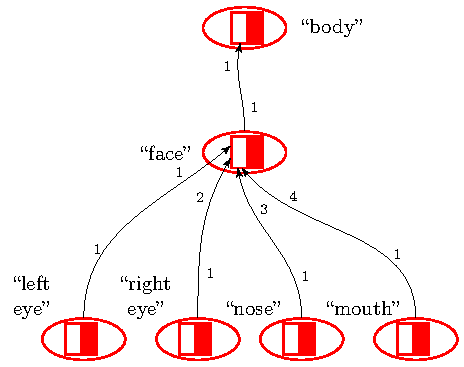
\includegraphics[page=1,width=0.55\textwidth]{examples/causnet/caus_net_colored_en}
		\includegraphics[width=0.4\textwidth]{misc/photos/face}
		
		\nocite{*}
		\printbibliography[keyword={signopernew}, resetnumbers=true]
	\end{frame}
	
	\begin{frame}
	\frametitle{Causal network on significances}
	
	\begin{figure}
	\includegraphics[page=2,width=0.7\textwidth]{examples/causnet/caus_net_colored_en}
	\end{figure}
	
	\end{frame}
	
	\begin{frame}
	\frametitle{Causal network on personal meanings}
	
	\begin{figure}
	\includegraphics[page=3,width=0.7\textwidth]{examples/causnet/caus_net_colored_en}
	\end{figure}
	
	\end{frame}

	\begin{frame}{Sign and semiotic network}
		
		\begin{columns}
			\begin{column}{0.4\textwidth}
				\begin{center}
					\includegraphics[width=0.7\textwidth]{signs/en/sign_naming_colored_en}
					\includegraphics[width=0.8\textwidth]{signnet/signs_net}
					
				\end{center}
			\end{column}
			\begin{column}{0.6\textwidth}
				\scriptsize
				\textbf{Sign} $s(n)$ with name $n$ is the quadruple $\left\langle n,{{T}^{p}}(n),{{T}^{m}}(n),{{T}^{a}}(n) \right\rangle $ such that all the three ratios are satisfied: $\Psi _{a}^{p}\Psi _{m}^{a}\Psi _{p}^{m}({{T}^{p}}(n))={{T}^{p}}(n)$, $\Psi _{p}^{a}\Psi _{a}^{p}\Psi _{m}^{a}({{T}^{m}}(n))={{T}^{m}}(n)$ and $\Psi _{m}^{a}\Psi _{p}^{m}\Psi _{a}^{p}({{T}^{a}}(n))={{T}^{a}}(n)$, i.e., for any composition of linking functions the three tensors $({{T}^{p}}(n),{{T}^{m}}(n),{{T}^{a}}(n))$ is a stationary point.
				\par\medskip
				\textbf{Semiotic network} is the triple $\left\langle {{W}_{n}},\mathbf{W},\mathbf{\Psi },\mathbf{\Phi } \right\rangle $, where $\mathbf{W}=\{{{W}_{p}},{{W}_{m}},{{W}_{a}}\}$ is a family of causal networks on images, significances and personal meanings, $\mathbf{\Psi }=\{\Psi _{p}^{m},\Psi _{m}^{a},\Psi _{a}^{p}\}$ is a family of linking functions, $\mathbf{\Phi } $ is a family of rules of activity propagation in causal networks, ${{W}_{n}}=(N,{{R}_{n}})$ - a semantic network on the names, where the set of vertices $N$ is the set of names of characters $N=\{n:\Psi _{a}^{p}\Psi _{m}^{a}\Psi _{p}^{m}({{T}^{p}}(n))={{T}^{p}}(n)\}$, and a family of relationships ${{R}_{n}}$ sets to linguistic communication on the set sign names and is a translation of the relations on the set of sign components(collections ${{R}_{p}},{{R}_{m}},{{R}_{a}}$).
			\end{column}
		\end{columns}
		\nocite{*}
		\printbibliography[keyword={symbsign}, resetnumbers=true]
	\end{frame}
	\subsection{Networks on the components of the sign}
		\begin{frame}{Relationships on the set of images}
			\centering
			\includegraphics[page=1,width=0.8\textwidth]{sign-schemas/sign_relations}
			
			Image similarity
		\end{frame}	
		
		\begin{frame}{Relationships on the set of images}
		
		\begin{columns}
		\begin{column}{0.3\textwidth}
			\centering
			Image inclusion
			\par\bigskip
			\par\bigskip
			\par\bigskip
			\par\bigskip
			\par\bigskip
			Image opposition
			
		\end{column}
		\begin{column}{0.7\textwidth}
			\includegraphics[page=2,width=0.8\textwidth]{sign-schemas/sign_relations}
			
			\includegraphics[page=3,width=0.8\textwidth]{sign-schemas/sign_relations}
		\end{column}
		\end{columns}
		
		\end{frame}	
		
		\begin{frame}
		\frametitle{Relationships on the set of significances}
		\centering
		\includegraphics[page=4,width=0.7\textwidth]{sign-schemas/sign_relations}
		
		Script on significances
		\end{frame}	
		
		\begin{frame}
		\frametitle{Relationships on the set of personal meaning}
		
		\begin{columns}
		\begin{column}{0.3\textwidth}
		\centering
		Agglutination of personal meanings
		\par\bigskip
		\par\bigskip
		\par\bigskip
		\par\bigskip
		\par\bigskip
		Opposition of personal meanings
		
		\end{column}
		\begin{column}{0.7\textwidth}
		\includegraphics[page=5,width=0.8\textwidth]{sign-schemas/sign_relations}
		\par\bigskip
		\includegraphics[page=6,width=0.8\textwidth]{sign-schemas/sign_relations}
		\end{column}
		\end{columns}
		\end{frame}	
	\subsection{Control role of the name}
	\begin{frame}{Network on sign names}
		\centering
		\includegraphics[width=0.7\textwidth]{signs/en/sign_levels_en}
		
		\nocite{*}
		\printbibliography[keyword={swm}, resetnumbers=true]
	\end{frame}	

	\subsection{Activity propogation}
	\begin{frame}{Local rules of activity propogation} 
		\scriptsize                            
		\begin{center}
			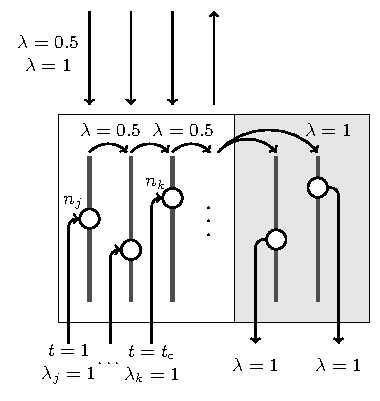
\includegraphics[width=0.27\textwidth]{causnet/caus_active}
		\end{center}

		\begin{itemize}
			\item \textit{The upward rule}: if at time $t$ the tensor $T({{n}_{j}})$ such that ${{n}_{j}}\in \bar{n}$ and ${{\lambda }_{j}}=1$, then all nonzero elements of $(j,t,{{\tau }_{l}})$ tensor $T({{n}_{i}})$ in each precedent of ${{\tau }_{l}}$ becomes active, i.e., ${{\lambda }_{jtl}}=1$.
			\item \textit{The predicting rule}: if at time $t$, the event ${{e}_{t}}$ of the precedent ${{\tau }_{l}}$ in the tensor $T({{n}_{i}})$ is active (i.e., $\forall f_{k}^{t}\in {{e}_{t}}:f_{k}^{t}>0\wedge {{\lambda }_{ktl}}=1$) and $t<{{t}_{c}}$, then all nonzero elements of $(k,t+1,{{\tau }_{l}})$ events in ${{e}_{t+1}}$ be a semi-active, i.e., ${{\lambda }_{jt+1l}}=0.5$.
			\item \textit{The downward rule}: if at time $t$ in each active precedent (i.e. $\forall u>0:u\le t$ is ${{e}_{u}}$ - active) tensor $T({{n}_{i}})$, the event ${{e}_{t}}$ - active (i.e., $\forall f_{k}^{t}\in {{e}_{t}}:f_{k}^{t}>0\wedge {{\lambda }_{ktl}}=1$), then all tensors $T({{n}_{j}})$ corresponding to the nonzero elements of $(j,t+1,{{\tau }_{l}})$ events in ${{e}_{t+1}}$ in each precedent of ${{\tau }_{l}}$ becomes semi-active.
			\item \textit{The causal rule}: if $t={{t}_{c}}$ event ${{e}_{{{t}_{c}}}}$ is active at the time, then the predictive rule and the downward rule are applied consistently for all effect events, adjusted for the fact that full activity is propagated, i.e. ${{\lambda }_{jtl}}=$1.
		\end{itemize}
		\vspace{-5pt}
		\nocite{*}
		\printbibliography[keyword={per}, resetnumbers=true]
	\end{frame}

	\begin{frame}{The model of the cognitive function}
		\begin{center}
			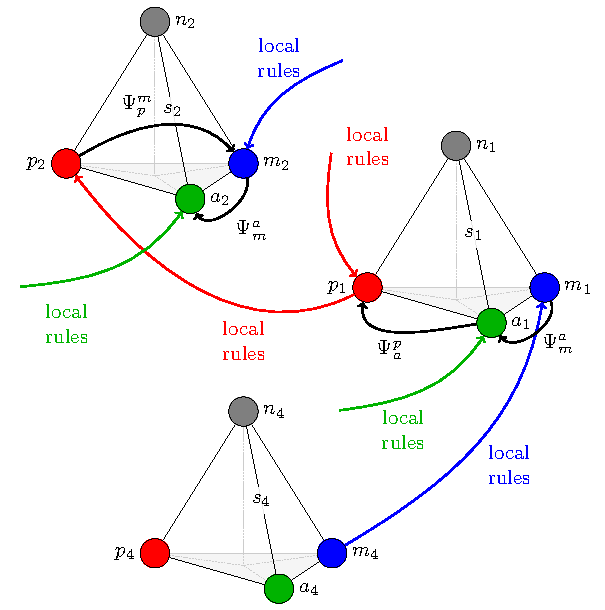
\includegraphics[width=0.4\textwidth]{sign-schemas/cognitive_function}
		\end{center}
		\textit{A cognitive function model} is the sequence of signs $({s}_{1}, {s}_{2},\dots)$ such that $\forall {{s}_{i}}({{n}_{i}})$ tensors for each component in ${{T}^{p}}({{n}_{i}}),{{T}^{m}}({{n}_{i}}),{{T}^{a}}({{n}_{i}})$ are simultaneously active, i.e. the propogation of activity leads to the activation of these causal tensors, which form a sign on each stage of the activity propogation.
	\end{frame}

	\subsection{Example of functions: categorization}
		\begin{frame}{Perception and categorization}
	
		\begin{tikzpicture}[overlay,remember picture]
		
		\tikzstyle{z_matrix} = [draw, rectangle, minimum width = 60, minimum height = 60,fill=white];
		
		\onslide<1->{
			\node (meas_fun) at (0.7,0.5) {$\hat f_1,\hat f_2\dots,\hat f_k$};	
		}
		\onslide<2->{
			\node (control_vect) at ($(meas_fun)+(-0.5,1.2)$) {$\hat x^{j+1}$};
			\path[->,thick,red] (control_vect.east)  edge[out = -45, in = 45, right] (meas_fun.north); 
		}
		\onslide<3->{
			\node[z_matrix] (z_1) at ($(meas_fun)+(2.6,-0.5)$) {};
			\node[z_matrix] at ($(z_1)+(0.2,-0.1)$) {};
			\node[z_matrix] at ($(z_1)+(0.4,-0.2)$) {};
			
			\node[z_matrix] at ($(z_1)+(0.9,-0.5)$) {};
			\node[z_matrix] at ($(z_1)+(1.1,-0.6)$) {};
			\node[z_matrix] at ($(z_1)+(1.3,-0.7)$) {};
			
			\path[->,thick,blue] ([xshift=20]meas_fun.south)  edge[out = -90, in = -155, right] ($(z_1)+(-1,-1.2)$);
			\path[->,thick,blue] ([xshift=-25]meas_fun.south)  edge[out = -90, in = -155, right] ($(z_1)+(-0.1,-1.7)$);
			
			\node at ($(z_1)+(-1,1.4)$) {$Z^*$};
			
			\node at ($(z_1)+(0.8,1.4)$) {$Z_1$};
			\node at ($(z_1)+(1.4,1.2)$) {$\ddots$};
			\node at ($(z_1)+(2,0.9)$) {$Z_k$};
		}
		
		\onslide<4->{
			\draw[ultra thick, green!60!black] ($(z_1)+(-0.4,-1.1)$) -- ($(z_1)+(-0.4,0.6)$);
			\draw[ultra thick, green!60!black] ($(z_1)+(0.5,-1.6)$) -- node[right,black] {$z_1^r$} ($(z_1)+(0.5,0.1)$);
			
			\draw[->, thick, green!60!black] ($(z_1)+(-0.1,-3)$) -- node[right,black] {$\bar x(0)$} ($(z_1)+(-0.1,-2)$);
		}
		
		\onslide<5->{
			\node[z_matrix] (z_2) at ($(z_1)+(5,0)$) {};
			\node[z_matrix] at ($(z_2)+(0.2,-0.1)$) {};
			
			\node[z_matrix] at ($(z_2)+(0.9,-0.5)$) {};
			\node[z_matrix] at ($(z_2)+(1.3,-0.7)$) {};
			
			\node at ($(z_2)+(-1,1.4)$) {$Z^*$};
			\node at ($(z_2)+(0.8,1.4)$) {$Z_1$};
			\node at ($(z_2)+(1.4,1.2)$) {$\ddots$};
			\node at ($(z_2)+(2,0.9)$) {$Z_k$};
			
			\draw[->, ultra thick] ($(z_1)+(2.6,-0.6)$) -- node [above] {\scriptsize$\frac{\|\bar z_1^r-\bar x(0)\|}{\|\bar z_1^r\|+\|\bar x(0)\|}$} ($(z_1)+(3.7,-0.6)$);
			
			\draw[ultra thick, dotted, green!60!black] ($(z_2)+(-0.6,-1)$) -- ($(z_2)+(-0.6,0.7)$);
			\draw[ultra thick, dotted, green!60!black] ($(z_2)+(0.5,-1.6)$) -- ($(z_2)+(0.5,0.1)$);
		}
		
		\onslide<6->{
			\draw[->, thick, red] ($(z_2)+(0.3,1.4)$) -- node[right,black] {$\bar x^*(0)$} ($(z_2)+(0.3,3)$);
		}
		
		\onslide<7>{
			\draw[<-, thick, red] ($(z_2)+(-0.1,-3)$) -- node[right,black] {$\hat x^j(0)$} ($(z_2)+(-0.1,-2)$);
		}
		
		\onslide<7->{				
			\draw[ultra thick, green!60!black] ($(z_2)+(-0.4,-1)$) -- ($(z_2)+(-0.4,0.7)$);
			\draw[ultra thick, green!60!black] ($(z_2)+(0.7,-1.6)$) -- node[right,black] {$z_2^r$} ($(z_2)+(0.7,0.1)$);	
		}
		\onslide<8->{
			\draw[->, thick, green!60!black] ($(z_2)+(-0.1,-3)$) -- node[right,black] {$\bar x(1)$} ($(z_2)+(-0.1,-2)$);
		}
		
		\onslide<9->{
			\draw[->, ultra thick] ($(z_2)+(2.6,-0.6)$) -- node [above] {\scriptsize$\frac{\|\bar z_1^r-\bar x(1)\|}{\|\bar z_1^r\|+\|\bar x(1)\|}$} ($(z_2)+(3.7,-0.6)$);
		}
		\end{tikzpicture}
		
	\end{frame}	
	\subsection{Example of functions: planning}
	\begin{frame}{Schema of the algorithm MAP}
		
		\begin{columns}
			\begin{column}{0.55\textwidth}
				\includegraphics[width=\textwidth]{algo/en/beh_plan2_en}
				\vspace{-5pt}
				\nocite{*}
				\printbibliography[keyword={plan}, resetnumbers=true]
			\end{column}
			\begin{column}{0.45\textwidth}
				\small
				The hierarchical planning process begins with the finish situation and seeks to achieve the start situation.
				\par\bigskip
				MAP iteration:
				\begin{itemize}
					\item \textit{S-step} -- search of precedents of the action implementation for the current conditions,
					\item \text{M-step} -- find applicable actions on the significance network,
					\item \text{A-step} -- generation of personal meanings corresponding to the found significances,
					\item \text{P-step} -- construct a new current situation from the set of features of the conditions of the found actions.
					
				\end{itemize}
			\end{column}
		\end{columns}
		
	\end{frame}		

	\begin{frame}{The fragment of the significance network}
		\begin{columns}
		\begin{column}{0.7\textwidth}
			\centering
			\includegraphics[page=2,width=\textwidth]{examples/plan/plan_nets}
		\end{column}
		\begin{column}{0.3\textwidth}
			\centering
			\includegraphics[page=1,width=\textwidth]{examples/plan/block_world}
		\end{column}
		\end{columns}
	\end{frame}	
	
	\begin{frame}{Personal meaning network - start situation}
		
		\centering
		\includegraphics[page=3,width=0.7\textwidth]{examples/plan/plan_nets}
		\par\bigskip
		\includegraphics[page=2,width=0.5\textwidth]{examples/plan/block_world}
	\end{frame}	
	
	\begin{frame}{Personal meaning network - final situation}
		\begin{columns}
		\begin{column}{0.7\textwidth}
		\centering
		\includegraphics[page=1,width=\textwidth]{examples/plan/plan_nets}
		\end{column}
		\begin{column}{0.3\textwidth}
		\centering
		\includegraphics[page=1,width=\textwidth]{examples/plan/block_world}
		\end{column}
		\end{columns}
	\end{frame}	
	
	\begin{frame}{The fragment of the significance network}
		\begin{columns}
		\begin{column}{0.7\textwidth}
		\centering
		\includegraphics[page=5,width=\textwidth]{examples/plan/plan_nets}
		\end{column}
		\begin{column}{0.3\textwidth}
		\centering
		\includegraphics[page=3,width=\textwidth]{examples/plan/block_world}
		\end{column}
		\end{columns}
	\end{frame}
	\begin{frame}{Generation of the next situation}
		
		\begin{tikzpicture}[overlay,remember picture,xshift=165pt,yshift=-50pt]

		\onslide<1->{
			\tikzstyle{ell}=[draw, thick, align=center, color=blue]
			\tikzstyle{ellf}=[draw, thick, align=center, color=blue, fill=blue]
			
			\node[ell, ellipse, minimum height = 30, minimum width = 100] (block) at (5 pt,0){};
			\predmatr{-30}{0}{block1}
			\predmatr{-10}{0}{block2}
			\predmatr{10}{0}{block3}	
			\predmatr{30}{0}{block4}
			\node at (35 pt, 20 pt) {``block''};
			
			\node[ell, ellipse, minimum height = 20, minimum width = 40] (c) at (32.5 pt, -50 pt){};
			\predmatr{30}{-50}{c1}
			\node at (10 pt, -35 pt) {``c''};		
			
			\node[ell, ellipse, minimum height = 20, minimum width = 40] (d) at (82.5 pt, -50 pt){};
			\predmatr{80}{-50}{d1}			
			\node at (60 pt, -35 pt) {``d''};	
			
			\node[ell, ellipse, minimum height = 20, minimum width = 40] (x) at (-37.5 pt, 50 pt){};
			\predmatr{-40}{50}{x1}
			\node at (-85 pt, 50 pt) {``block?x''};			
			
			\node[ell, ellipse, minimum height = 20, minimum width = 40] (y) at (42.5 pt, 50 pt){};
			\predmatr{40}{50}{y1}	
			\node at (85 pt, 50 pt) {``block?y''};
			
			\path[-latex'] (c.north) edge [out = 90, in = -80] node[above, black] {\scriptsize 1} node[above, black, near start] {\scriptsize 1} ([xshift=-3]block3.south);
			\path[-latex'] (d.north) edge [out = 90, in = -80] node[above, black, near end] {\scriptsize 1} node[above, black, near start] {\scriptsize 1} ([xshift=-3]block4.south);	
		}
		\onslide<1>{
			\node[ell, ellipse, minimum height = 20, minimum width = 40] (a) at (-77.5 pt, -50 pt){};
			\predmatr{-80}{-50}{a1}
			\node at (-100 pt, -35 pt) {``a''};
			
			\node[ell, ellipse, minimum height = 20, minimum width = 40] (b) at (-27.5 pt, -50 pt){};
			\predmatr{-30}{-50}{b1}
			\node at (-50 pt, -35 pt) {``b''};		
		}
		\onslide<1-2>{
			\path[-latex'] (a.north) edge [out = 90, in = -120] node[above, black, near end] {\scriptsize 1} node[above, black, near start] {\scriptsize 1} ([xshift=-3]block1.south);
			\path[-latex'] (b.north) edge [out = 90, in = -120] node[above, black, near end] {\scriptsize 1} node[above, black, near start] {\scriptsize 1} ([xshift=-3]block2.south);
		}			
		\onslide<1-3>{
			\path[-latex'] ([xshift=-10]block.north) edge [out = 90, in = -80] node[above, black] {\scriptsize 1} node[above, black, near start] {\scriptsize 0} ([xshift=-3]x1.south);
			\path[-latex'] ([xshift=10]block.north) edge [out = 90, in = -100] node[above, black] {\scriptsize 1} node[above, black, near start] {\scriptsize 0} ([xshift=-3]y1.south);
		}
		\onslide<1-4>{
			\node[ell, ellipse, minimum height = 20, minimum width = 40] (unstack) at (2.5 pt, 100 pt){};
			\predmatr{0}{100}{unstack1}
			\node at (-15 pt, 120 pt) {``unstack''};
			
			\node[ell, ellipse, minimum height = 20, minimum width = 40] (on) at (-77.5 pt, 100 pt){};
			\predmatr{-80}{100}{on1}
			\node at (-115 pt, 100 pt) {``on''};
			
			\path[-latex'] (x.north) edge [out = 90, in = -100] node[above, black, near end] {\scriptsize -1} node[above, black, near start] {\scriptsize 1} ([xshift=2]unstack1.south);
			\path[-latex'] (y.north) edge [out = 90, in = -80] node[above, black, near end] {\scriptsize -2} node[above, black, near start] {\scriptsize 1} ([xshift=5]unstack1.south);
			\path[-latex'] (on.east) edge [out = 0, in = 180] node[above, black, near end] {\scriptsize 1} node[above, black, near start] {\scriptsize 1} ([yshift=-3]unstack1.west);
			
			\path[-latex'] ([xshift=-10]x.north) edge [out = 100, in = -140] node[above, black] {\scriptsize 1} node[above, black, very near start] {\scriptsize 1} ([xshift=-3]on1.south);	
			\path[-latex'] ([xshift=-10]y.north) edge [out = 150, in = -30] node[above, black, near end] {\scriptsize -1} node[above, black, very near start] {\scriptsize 1} ([xshift=3]on1.south);					
		}			
		\onslide<1-5>{
			\node[ell, ellipse, minimum height = 20, minimum width = 40] (holding) at (82.5 pt, 120 pt){};
			\predmatr{80}{120}{holding1}
			\node at (125 pt, 120 pt) {``holding''};
			
			\node[ell, ellipse, minimum height = 20, minimum width = 40] (clear) at (82.5 pt, 90 pt){};
			\predmatr{80}{90}{clear1}
			\node at (120 pt, 90 pt) {``clear''};
			
			\path[-latex'] (clear.west) edge [out = 180, in = 0] node[above, black, near end] {\scriptsize -2} node[above, black, near start] {\scriptsize 1} ([yshift=-3]unstack1.east);
			\path[-latex'] (holding.west) edge [out = 180, in = 0] node[above, black, near end] {\scriptsize -1} node[above, black, near start] {\scriptsize 1} ([yshift=3]unstack1.east);
			
		}
		\onslide<2->{
			\tikzstyle{ell}=[draw, thick, align=center, color=green!70!black]
			\tikzstyle{ellf}=[draw, thick, align=center, color=green!70!black, fill=green!70!black]
			
			\node[ell, ellipse, minimum height = 20, minimum width = 40] (a) at (-77.5 pt, -50 pt){};
			\predmatr{-80}{-50}{a1}
			\node at (-100 pt, -35 pt) {``a''};
			
			\node[ell, ellipse, minimum height = 20, minimum width = 40] (b) at (-27.5 pt, -50 pt){};
			\predmatr{-30}{-50}{b1}
			\node at (-50 pt, -35 pt) {``b''};
		}
		\onslide<3->{
			\path[-latex', very thick] (a.north) edge [out = 90, in = -120] node[above, black, near end] {\scriptsize 1} node[above, black, near start] {\scriptsize 1} ([xshift=-3]block1.south);
			\path[-latex', very thick] (b.north) edge [out = 90, in = -120] node[above, black, near end] {\scriptsize 1} node[above, black, near start] {\scriptsize 1} ([xshift=-3]block2.south);	
		}
		\onslide<4->{
			\path[-latex', very thick] ([xshift=-10]block.north) edge [out = 90, in = -80] node[above, black] {\scriptsize 1} node[above, black, near start] {\scriptsize 0} ([xshift=-3]x1.south);
			\path[-latex', very thick] ([xshift=10]block.north) edge [out = 90, in = -100] node[above, black] {\scriptsize 1} node[above, black, near start] {\scriptsize 0} ([xshift=-3]y1.south);
		}
		\onslide<5->{
			\node[ell, ellipse, minimum height = 20, minimum width = 40] (unstack) at (2.5 pt, 100 pt){};
			\predmatr{0}{100}{unstack1}
			\node at (-15 pt, 120 pt) {``unstack''};
			
			\node[ell, ellipse, minimum height = 20, minimum width = 40] (on) at (-77.5 pt, 100 pt){};
			\predmatr{-80}{100}{on1}
			\node at (-115 pt, 100 pt) {``on''};
			
			\path[-latex', very thick] (on.east) edge [out = 0, in = 180] node[above, black, near end] {\scriptsize 1} node[above, black, near start] {\scriptsize 1} ([yshift=-3]unstack1.west);
			
			\path[-latex', very thick] ([xshift=-10]x.north) edge [out = 100, in = -140] node[above, black] {\scriptsize 1} node[above, black, very near start] {\scriptsize 1} ([xshift=-3]on1.south);	
			\path[-latex', very thick] ([xshift=-10]y.north) edge [out = 150, in = -30] node[above, black, near end] {\scriptsize -1} node[above, black, very near start] {\scriptsize 1} ([xshift=3]on1.south);
			\path[-latex', very thick] (x.north) edge [out = 90, in = -100] node[above, black, near end] {\scriptsize -1} node[above, black, near start] {\scriptsize 1} ([xshift=2]unstack1.south);
			\path[-latex', very thick] (y.north) edge [out = 90, in = -80] node[above, black, near end] {\scriptsize -2} node[above, black, near start] {\scriptsize 1} ([xshift=5]unstack1.south);	
		}
		\onslide<6->{
			\node[ell, ellipse, minimum height = 20, minimum width = 40] (holding) at (82.5 pt, 120 pt){};
			\predmatr{80}{120}{holding1}
			\node at (125 pt, 120 pt) {``holding''};
			
			\node[ell, ellipse, minimum height = 20, minimum width = 40] (clear) at (82.5 pt, 90 pt){};
			\predmatr{80}{90}{clear1}
			\node at (120 pt, 90 pt) {``clear''};
			
			\path[-latex', very thick] (clear.west) edge [out = 180, in = 0] node[above, black, near end] {\scriptsize -2} node[above, black, near start] {\scriptsize 1} ([yshift=-3]unstack1.east);
			\path[-latex', very thick] (holding.west) edge [out = 180, in = 0] node[above, black, near end] {\scriptsize -1} node[above, black, near start] {\scriptsize 1} ([yshift=3]unstack1.east);
		}			
		\end{tikzpicture}
	\end{frame}	

	\begin{frame}
		\frametitle{The current situation}
		\begin{columns}
			\begin{column}{0.7\textwidth}
				\centering
				\includegraphics[page=4,width=\textwidth]{examples/plan/plan_nets}
			\end{column}
			\begin{column}{0.3\textwidth}
				\centering
				\includegraphics[page=3,width=\textwidth]{examples/plan/block_world}
			\end{column}
		\end{columns}
	\end{frame}

	\begin{frame}{Formation of the new sign}
	
		Formation of a new rule and learning a new sign - formation of new causal matrices.
		\par\bigskip
		\centering
		\includegraphics[page=6,width=0.6\textwidth]{examples/plan/plan_nets}
		\includegraphics[page=7,width=0.4\textwidth]{examples/plan/plan_nets}
	\end{frame}
	

	\subsection{Example of functions: goal-setting}
	\begin{frame}{Goal-setting on the syntactic level}
		\begin{center}
			\includegraphics[width=0.8\textwidth]{algo/en/goal_set_alg_en}
		\end{center}
		\end{frame}

	\begin{frame}{Goal-setting in planning}
		\begin{center}
			\includegraphics[width=0.9\textwidth]{algo/en/gmap_en}
		\end{center}
		\vspace{-5pt}
		\nocite{*}
		\printbibliography[keyword={goalres}, resetnumbers=true]
	\end{frame}

	\subsection{Learning: formation of the sign}
	
	\begin{frame}{Iterative and unsupervised learning}
		We construct an algorithm $\mathfrak A_{pm}$ to determine the function $\Psi_p^m$, which provides the formation of such an image from the set of features $\hat F$, in which the generated sign value converges to the given value $\tilde m^0=\{f_p^0\}$.
		\par\bigskip
		The proposed learning algorithm is based on the hierarchical temporal memory (HTM) approach and consists of the following basic steps:
		\begin{enumerate}
			\item Formation of spatial representation.
			\item Search for time sequences.
			\item Identification of the causal relationship.
		\end{enumerate}
		
		\nocite{*}
		\printbibliography[keyword={signform}, resetnumbers=true]
	\end{frame}

	\section{Applied problems}
	\subsection{STRL architecture}
	
	\begin{frame}{Strategic,tactic,reactive layered architecture}
		\begin{center}
			\includegraphics[width=0.43\textwidth]{agent-schemas/en/strl_arch_real_eng}
		\end{center}
		\vspace{-5pt}
		\nocite{*}
		\printbibliography[keyword={strl}, resetnumbers=true]
	\end{frame}

	\subsection{Role distribution}
	\begin{frame}{Smart Relocation Tasks (SRT)}
		
		\begin{columns}
			\small
			\begin{column}{0.6\textwidth}
				\begin{center}
					\includegraphics[page=1,width=0.7\textwidth]{examples/plan/slides_colored}
				\end{center}
				
				\textbf{Problem}
				
				Goal area can not be achieved by some agents on their own (using standalone task and path planning methods)
				
				\textbf{Solution}
				
				Agents must communicate and some agents must alter their ``selfish'' plans in order to construct coalition plan
				
			\end{column}
			\begin{column}{0.4\textwidth}
				3 levels of control:
				\begin{itemize}
					\item Transformable environment
					\item Different types of obstacles (some -- can be destroyed)
					\item Agents with different capabilities (some agents can destroy obstacles, others -- can not)
					\item Common spatial goal (ALL agents must reach this region in order goal to be achieved)
				\end{itemize}
			\end{column}
		\end{columns}
		\vspace{-5pt}
		\nocite{*}
		\printbibliography[keyword={srt}, resetnumbers=true]
		\end{frame}
		
		\begin{frame}{Spatial knowledge representation}
		
			\begin{figure}
			\includegraphics[width=\textwidth]{examples/representations/rita_ex_proc.png}
			\end{figure}
		\end{frame}
		
		\begin{frame}{Spatial knowledge representation}
		
			Relocation actions --- signs $s_t$ (features $f_t$, $t$ --- relocation type), with corresponding prediction matrices $Z_t$ consist of 3 columns:
			\[
			z_1=(l_x, I), z_2=(l_y, d_u, E), z_3=(l_y, I, t_v),
			\]
			\begin{itemize}
			\item $l_x$, $l_y$ --- features represented category of distance in a spatial logic (e.g., ``far'', ``closely'' etc.), 
			\item $d_u$ --- features represented category of direction in a spatial logic (e.g., ``left'', ``straight'' etc.), 
			\item $t_v$ --- features represented category of time in temporal logic (e.g., ``soon'', ``not soon'' etc.),
			\item $I$ --- feature of agent presence, 
			\item $E$ --- feature of obstacle absence.
			\end{itemize}
			\vspace{-5pt}
			\nocite{*}
			\printbibliography[keyword={spatial}, resetnumbers=true]
		\end{frame}
		\begin{frame}{Spatial knowledge representation}
			
			\begin{columns}
				\begin{column}{0.55\textwidth}
					\includegraphics[width=\textwidth]{examples/representations/spatial_swm.jpg}
				\end{column}
				\begin{column}{0.45\textwidth}
					\includegraphics[width=\textwidth]{examples/representations/areas_signif.jpg}
				\end{column}
			\end{columns}
		\end{frame}
		\begin{frame}{Model scenario of interaction}
			\begin{center}
			\scalebox{0.7}{
			\animategraphics{12}{examples/plan/slides_colored}{}{}			
			}
			\end{center}
		\end{frame}
		\begin{frame}{Robotic implementation}
		
		\begin{columns}
			\begin{column}{0.6\textwidth}
				\centering
				\includegraphics[width=0.6\textwidth]{misc/robots/gazebo.jpg}
				\includegraphics[width=\textwidth]{misc/robots/maplib.png}
			\end{column}
			\begin{column}{0.4\textwidth}
				\includegraphics[width=\textwidth]{misc/robots/nexus.jpg}
				\par\bigskip
				\url{https://github.com/cog-isa/map-planner}
			\end{column}
		\end{columns}
	\end{frame}
	\subsection{Reinforcement learning}
	\begin{frame}{Reinforcement for formation of\\causal matrices}
		\footnotesize
		
		\begin{columns}
			\begin{column}{0.5\textwidth}
				\centering
				\includegraphics[width=0.7\textwidth]{rl/schema.png}
			\end{column}
			\begin{column}{0.5\textwidth}
				\includegraphics[width=0.8\textwidth]{rl/autoham.png}
			\end{column}
		\end{columns}
		
		
		\begin{itemize}
			\item \textbf{Hierarchical reinforcement learning} to form representation of new actions.
			\item The alternation of the processes of action abstraction and abstraction of states of the environment.
			\item Automatic formation of the hierarchy of operations.
		\end{itemize}
		\vspace{-5pt}
		\nocite{*}
		\printbibliography[keyword={ham}, resetnumbers=true]
	\end{frame}	
		\begin{frame}{Anomaly detection}
		\footnotesize
		
		\begin{columns}
			\begin{column}{0.5\textwidth}
				\centering
				\includegraphics[width=0.45\textwidth]{misc/mpf/schema.jpg}
			\end{column}
			\begin{column}{0.5\textwidth}
				\centering
				\includegraphics[width=0.45\textwidth]{misc/mpf/anom1.jpg}
				\vspace{10pt}
				\includegraphics[width=0.45\textwidth]{misc/mpf/anom2.jpg}
			\end{column}
		\end{columns}
		Preprocessing:
		\begin{itemize}
			\item Image loading.
			\item Algorithms which control the sensor's movement around the image.
		\end{itemize}
		Score computing:
		\[
		score = \frac{\sum_{i=0}^n \left(ac_{expected}^{(i)}-ac_{real}^{(i)}\right)^2}{n}
		\]
		\vspace{-5pt}
		\nocite{*}
		\printbibliography[keyword={anomaly}, resetnumbers=true]		
		\end{frame}	
	\subsection{Cognitive assistant}
		\begin{frame}{Assistant for education and health-care}
		
		\begin{figure}
			\includegraphics[width=\textwidth]{agent-schemas/en/cogasst_en}
		\end{figure}
	\end{frame}

	\section{Conclusion}
		\begin{frame}{Acknowledgments and team}
		
		\begin{figure}
			\includegraphics[width=\textwidth]{misc/photos/team_en.png}
		\end{figure}
	\end{frame}
	
	\begin{frame}{Publications}
		
		\nocite{*}
		\printbibliography[keyword={fulllist}, resetnumbers=true]
	\end{frame}

	\begin{frame}
	
		\centering
		\Huge
		Thank you for your attention!
		\normalsize
		\par\bigskip
		\par\bigskip
		Institute for AI Problems at FRC CSC RAS
		\par\bigskip
		Laboratory of Cognitive dynamic systems at MIPT
		\par\bigskip
		pan@isa.ru, panov.ai@mipt.ru
	\end{frame}			
\end{document}
	
	
